Die Markow-Eigenschaft, obwohl relativ simpel, erhält ein eigenes Kapitel, da sie von fundamentaler Wichtigkeit ist und bei der Modellierung eines Reinforcement Learning Problems eine besondere Rolle spielt. Verbinden lässt sich dies sehr gut mit einem Einblick über die grundsätzliche Modellierung von Zuständen bei einem Reinforcement Learning Problem.

\begin{quote}
    The future is independent of the past given the present
  \end{quote}

Dieser Satz erscheint oft in Büchern und Papern, wenn es um die Markov-Eigenschaft geht, denn er versucht zusammenzufassen, was diese aussagt. Im Zusammenhang von MDPs lässt sich dieser Satz so übersetzen, dass ein Folgezustand nicht abhängig von Aktionen bzw. Zuständen in der Vergangenheit ist, sondern ausschließlich von dem aktuellen Zustand und der aktuell gewählten Aktion.
In der Literatur gibt es unterschiedliche Auffassungen darüber, ob die Markov-Eigenschaft an den MDP direkt geknüpft ist oder an den Zustand, den der Agent zur Abwägung der Entscheidung zur Verfügung hat. Bei der ersten Annahme wird davon ausgegangen, dass der Zustand, der von der Umwelt ausgeliefert wird direkt die Markov-Eigenschaft besitzen muss. (Sutton S.49) hingegen bindet die Eigenschaft an den Zustand und nicht an den Entscheidungsprozess als solches. Ein Zustand ist somit die Menge aller notwendigen Informationen der Vergangenheit, die für die Zukunft relevant sind. Statt den gegebenen Zustand der Umwelt direkt zu übernehmen, werden hier Beobachtungen der Umwelt zu einer internen Repräsentation von Markov-Zuständen verarbeitet.


% \begin{figure}[H]
%     \centering
%     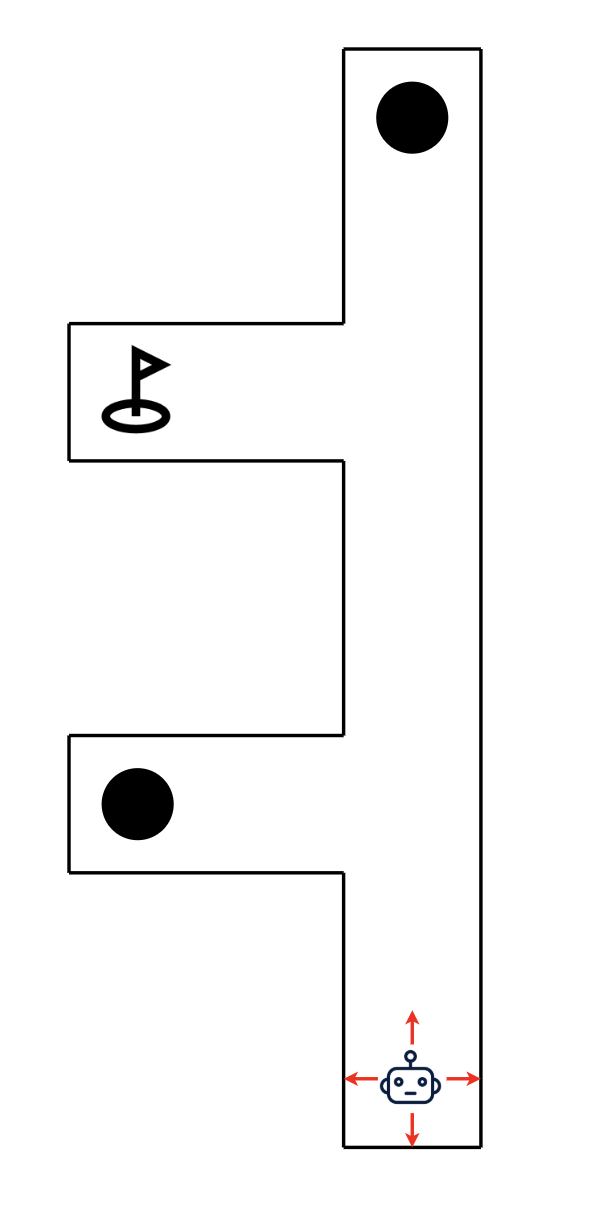
\includegraphics[height=250px]{images/2passagesDefault.png}
%     \caption{ Zwei-Wege Beispiel zu der Markov-Eigenschaft}
% \end{figure}

% \begin{wrapfigure}{L}{0.5\textwidth}
%   \begin{center}
%   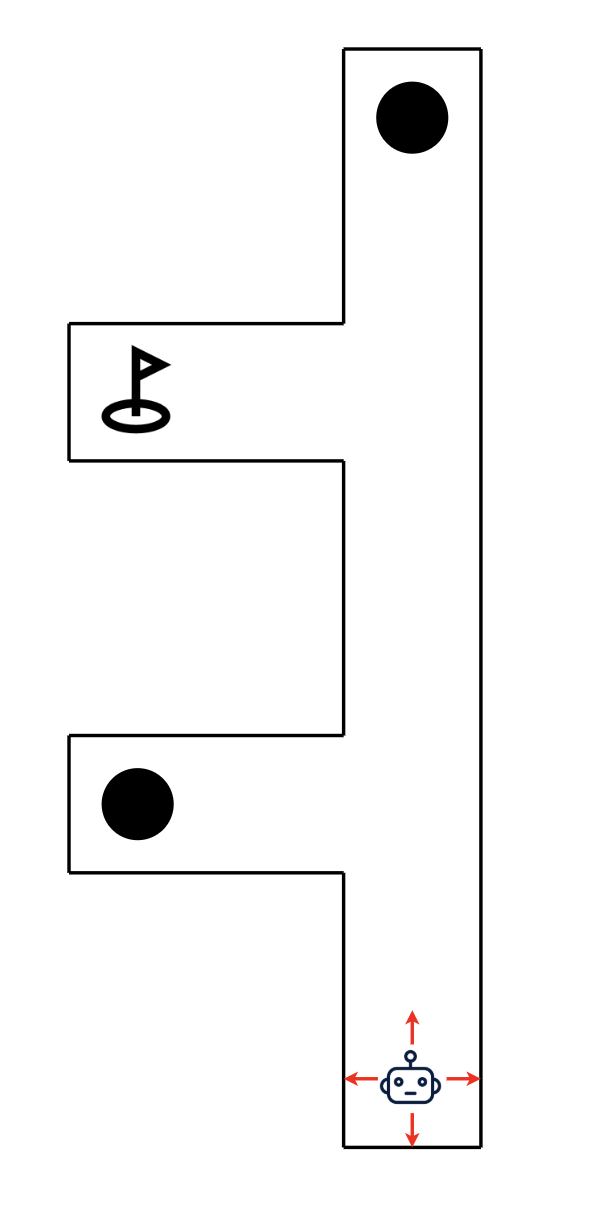
\includegraphics[height=250px]{images/2passagesDefault.png}  \end{center}
%   \caption{Birds}
% \end{wrapfigure}
